\documentclass[1p]{elsarticle_modified}
%\bibliographystyle{elsarticle-num}

%\usepackage[colorlinks]{hyperref}
%\usepackage{abbrmath_seonhwa} %\Abb, \Ascr, \Acal ,\Abf, \Afrak
\usepackage{amsfonts}
\usepackage{amssymb}
\usepackage{amsmath}
\usepackage{amsthm}
\usepackage{scalefnt}
\usepackage{amsbsy}
\usepackage{kotex}
\usepackage{caption}
\usepackage{subfig}
\usepackage{color}
\usepackage{graphicx}
\usepackage{xcolor} %% white, black, red, green, blue, cyan, magenta, yellow
\usepackage{float}
\usepackage{setspace}
\usepackage{hyperref}

\usepackage{tikz}
\usetikzlibrary{arrows}

\usepackage{multirow}
\usepackage{array} % fixed length table
\usepackage{hhline}

%%%%%%%%%%%%%%%%%%%%%
\makeatletter
\renewcommand*\env@matrix[1][\arraystretch]{%
	\edef\arraystretch{#1}%
	\hskip -\arraycolsep
	\let\@ifnextchar\new@ifnextchar
	\array{*\c@MaxMatrixCols c}}
\makeatother %https://tex.stackexchange.com/questions/14071/how-can-i-increase-the-line-spacing-in-a-matrix
%%%%%%%%%%%%%%%

\usepackage[normalem]{ulem}

\newcommand{\msout}[1]{\ifmmode\text{\sout{\ensuremath{#1}}}\else\sout{#1}\fi}
%SOURCE: \msout is \stkout macro in https://tex.stackexchange.com/questions/20609/strikeout-in-math-mode

\newcommand{\cancel}[1]{
	\ifmmode
	{\color{red}\msout{#1}}
	\else
	{\color{red}\sout{#1}}
	\fi
}

\newcommand{\add}[1]{
	{\color{blue}\uwave{#1}}
}

\newcommand{\replace}[2]{
	\ifmmode
	{\color{red}\msout{#1}}{\color{blue}\uwave{#2}}
	\else
	{\color{red}\sout{#1}}{\color{blue}\uwave{#2}}
	\fi
}

\newcommand{\Sol}{\mathcal{S}} %segment
\newcommand{\D}{D} %diagram
\newcommand{\A}{\mathcal{A}} %arc


%%%%%%%%%%%%%%%%%%%%%%%%%%%%%5 test

\def\sl{\operatorname{\textup{SL}}(2,\Cbb)}
\def\psl{\operatorname{\textup{PSL}}(2,\Cbb)}
\def\quan{\mkern 1mu \triangleright \mkern 1mu}

\theoremstyle{definition}
\newtheorem{thm}{Theorem}[section]
\newtheorem{prop}[thm]{Proposition}
\newtheorem{lem}[thm]{Lemma}
\newtheorem{ques}[thm]{Question}
\newtheorem{cor}[thm]{Corollary}
\newtheorem{defn}[thm]{Definition}
\newtheorem{exam}[thm]{Example}
\newtheorem{rmk}[thm]{Remark}
\newtheorem{alg}[thm]{Algorithm}

\newcommand{\I}{\sqrt{-1}}
\begin{document}

%\begin{frontmatter}
%
%\title{Boundary parabolic representations of knots up to 8 crossings}
%
%%% Group authors per affiliation:
%\author{Yunhi Cho} 
%\address{Department of Mathematics, University of Seoul, Seoul, Korea}
%\ead{yhcho@uos.ac.kr}
%
%
%\author{Seonhwa Kim} %\fnref{s_kim}}
%\address{Center for Geometry and Physics, Institute for Basic Science, Pohang, 37673, Korea}
%\ead{ryeona17@ibs.re.kr}
%
%\author{Hyuk Kim}
%\address{Department of Mathematical Sciences, Seoul National University, Seoul 08826, Korea}
%\ead{hyukkim@snu.ac.kr}
%
%\author{Seokbeom Yoon}
%\address{Department of Mathematical Sciences, Seoul National University, Seoul, 08826,  Korea}
%\ead{sbyoon15@snu.ac.kr}
%
%\begin{abstract}
%We find all boundary parabolic representation of knots up to 8 crossings.
%
%\end{abstract}
%\begin{keyword}
%    \MSC[2010] 57M25 
%\end{keyword}
%
%\end{frontmatter}

%\linenumbers
%\tableofcontents
%
\newcommand\colored[1]{\textcolor{white}{\rule[-0.35ex]{0.8em}{1.4ex}}\kern-0.8em\color{red} #1}%
%\newcommand\colored[1]{\textcolor{white}{ #1}\kern-2.17ex	\textcolor{white}{ #1}\kern-1.81ex	\textcolor{white}{ #1}\kern-2.15ex\color{red}#1	}

{\Large $\underline{12n_{0314}~(K12n_{0314})}$}

\setlength{\tabcolsep}{10pt}
\renewcommand{\arraystretch}{1.6}
\vspace{1cm}\begin{tabular}{m{100pt}>{\centering\arraybackslash}m{274pt}}
\multirow{5}{120pt}{
	\centering
	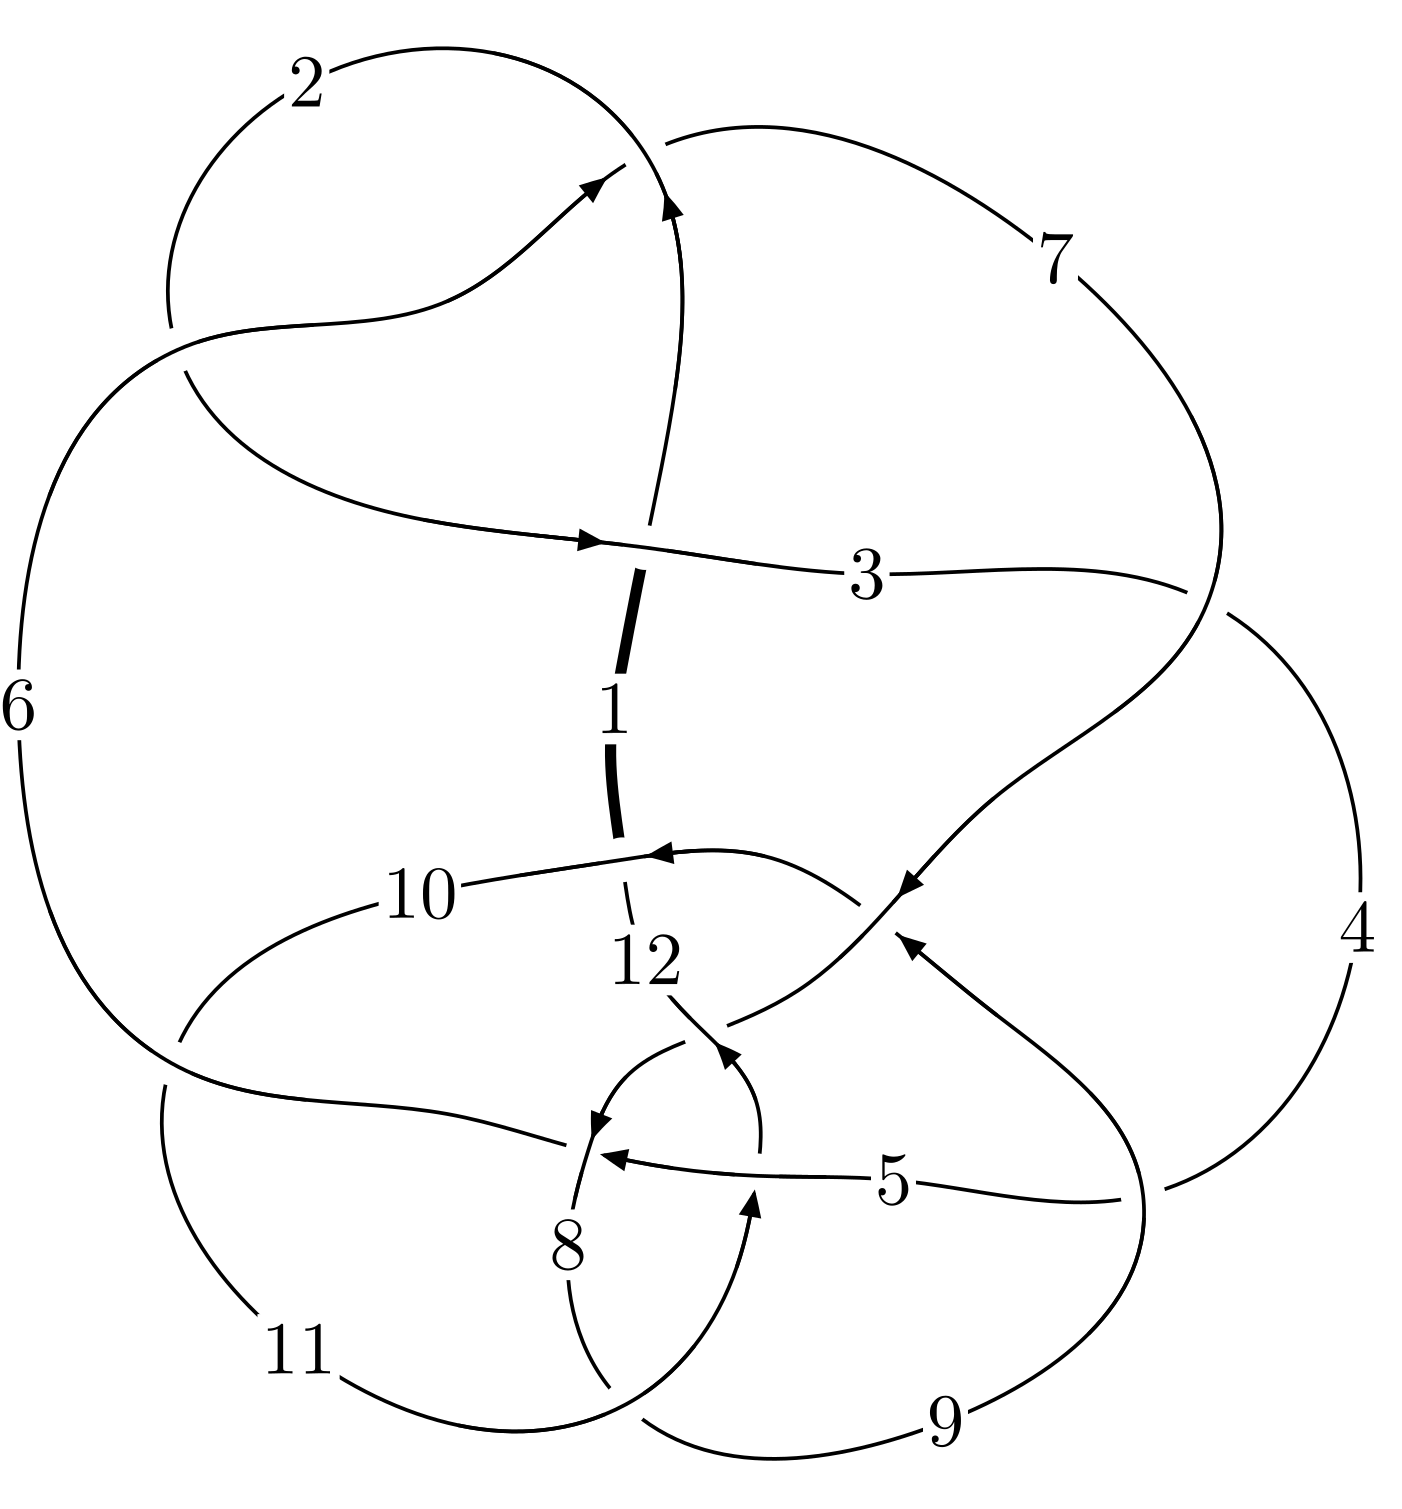
\includegraphics[width=112pt]{../../../GIT/diagram.site/Diagrams/png/2403_12n_0314.png}\\
\ \ \ A knot diagram\footnotemark}&
\allowdisplaybreaks
\textbf{Linearized knot diagam} \\
\cline{2-2}
 &
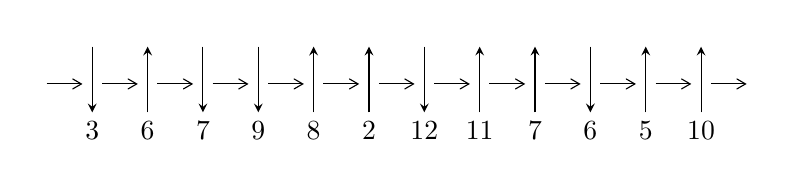
\begin{tikzpicture}[x=20pt, y=17pt]
	% nodes
	\node (C0) at (0, 0) {};
	\node (C1) at (1, 0) {};
	\node (C1U) at (1, +1) {};
	\node (C1D) at (1, -1) {3};

	\node (C2) at (2, 0) {};
	\node (C2U) at (2, +1) {};
	\node (C2D) at (2, -1) {6};

	\node (C3) at (3, 0) {};
	\node (C3U) at (3, +1) {};
	\node (C3D) at (3, -1) {7};

	\node (C4) at (4, 0) {};
	\node (C4U) at (4, +1) {};
	\node (C4D) at (4, -1) {9};

	\node (C5) at (5, 0) {};
	\node (C5U) at (5, +1) {};
	\node (C5D) at (5, -1) {8};

	\node (C6) at (6, 0) {};
	\node (C6U) at (6, +1) {};
	\node (C6D) at (6, -1) {2};

	\node (C7) at (7, 0) {};
	\node (C7U) at (7, +1) {};
	\node (C7D) at (7, -1) {12};

	\node (C8) at (8, 0) {};
	\node (C8U) at (8, +1) {};
	\node (C8D) at (8, -1) {11};

	\node (C9) at (9, 0) {};
	\node (C9U) at (9, +1) {};
	\node (C9D) at (9, -1) {7};

	\node (C10) at (10, 0) {};
	\node (C10U) at (10, +1) {};
	\node (C10D) at (10, -1) {6};

	\node (C11) at (11, 0) {};
	\node (C11U) at (11, +1) {};
	\node (C11D) at (11, -1) {5};

	\node (C12) at (12, 0) {};
	\node (C12U) at (12, +1) {};
	\node (C12D) at (12, -1) {10};
	\node (C13) at (13, 0) {};

	% arrows
	\draw[->,>={angle 60}]
	(C0) edge (C1) (C1) edge (C2) (C2) edge (C3) (C3) edge (C4) (C4) edge (C5) (C5) edge (C6) (C6) edge (C7) (C7) edge (C8) (C8) edge (C9) (C9) edge (C10) (C10) edge (C11) (C11) edge (C12) (C12) edge (C13) ;	\draw[->,>=stealth]
	(C1U) edge (C1D) (C2D) edge (C2U) (C3U) edge (C3D) (C4U) edge (C4D) (C5D) edge (C5U) (C6D) edge (C6U) (C7U) edge (C7D) (C8D) edge (C8U) (C9D) edge (C9U) (C10U) edge (C10D) (C11D) edge (C11U) (C12D) edge (C12U) ;
	\end{tikzpicture} \\
\hhline{~~} \\& 
\textbf{Solving Sequence} \\ \cline{2-2} 
 &
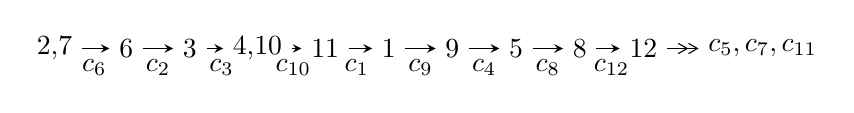
\begin{tikzpicture}[x=23pt, y=7pt]
	% node
	\node (A0) at (-1/8, 0) {2,7};
	\node (A1) at (1, 0) {6};
	\node (A2) at (2, 0) {3};
	\node (A3) at (49/16, 0) {4,10};
	\node (A4) at (33/8, 0) {11};
	\node (A5) at (41/8, 0) {1};
	\node (A6) at (49/8, 0) {9};
	\node (A7) at (57/8, 0) {5};
	\node (A8) at (65/8, 0) {8};
	\node (A9) at (73/8, 0) {12};
	\node (C1) at (1/2, -1) {$c_{6}$};
	\node (C2) at (3/2, -1) {$c_{2}$};
	\node (C3) at (5/2, -1) {$c_{3}$};
	\node (C4) at (29/8, -1) {$c_{10}$};
	\node (C5) at (37/8, -1) {$c_{1}$};
	\node (C6) at (45/8, -1) {$c_{9}$};
	\node (C7) at (53/8, -1) {$c_{4}$};
	\node (C8) at (61/8, -1) {$c_{8}$};
	\node (C9) at (69/8, -1) {$c_{12}$};
	\node (A10) at (11, 0) {$c_{5},c_{7},c_{11}$};

	% edge
	\draw[->,>=stealth]	
	(A0) edge (A1) (A1) edge (A2) (A2) edge (A3) (A3) edge (A4) (A4) edge (A5) (A5) edge (A6) (A6) edge (A7) (A7) edge (A8) (A8) edge (A9) ;
	\draw[->>,>={angle 60}]	
	(A9) edge (A10);
\end{tikzpicture} \\ 

\end{tabular} \\

\footnotetext{
The image of knot diagram is generated by the software ``\textbf{Draw programme}" developed by Andrew Bartholomew(\url{http://www.layer8.co.uk/maths/draw/index.htm\#Running-draw}), where we modified some parts for our purpose(\url{https://github.com/CATsTAILs/LinksPainter}).
}\phantom \\ \newline 
\centering \textbf{Ideals for irreducible components\footnotemark of $X_{\text{par}}$} 
 
\begin{align*}
I^u_{1}&=\langle 
26419 u^{19}+221467 u^{18}+\cdots+81793 b+229898,\\
\phantom{I^u_{1}}&\phantom{= \langle  }655714 u^{19}+5585712 u^{18}+\cdots+1717653 a+17248644,\;u^{20}+9 u^{19}+\cdots+105 u+21\rangle \\
I^u_{2}&=\langle 
u^{14}-5 u^{13}+\cdots+13 b-16,\;3 u^{14}-2 u^{13}+\cdots+13 a+56,\;u^{15}+4 u^{14}+\cdots-4 u-1\rangle \\
I^u_{3}&=\langle 
179 u^6 a^3+84 u^6 a^2+\cdots+240 a-68,\;2 u^6 a^3+5 u^6 a^2+\cdots- a+5,\;u^7-2 u^6+2 u^5+u^2-2 u+1\rangle \\
I^u_{4}&=\langle 
b+u,\;a^2- a u+2 a+1,\;u^2- u+1\rangle \\
I^u_{5}&=\langle 
b- u+1,\;a^2- a u- a+u-1,\;u^2- u+1\rangle \\
\\
I^v_{1}&=\langle 
a,\;b^2+b+1,\;v+1\rangle \\
\end{align*}
\raggedright * 6 irreducible components of $\dim_{\mathbb{C}}=0$, with total 73 representations.\\
\footnotetext{All coefficients of polynomials are rational numbers. But the coefficients are sometimes approximated in decimal forms when there is not enough margin.}
\newpage
\renewcommand{\arraystretch}{1}
\centering \section*{I. $I^u_{1}= \langle 26419 u^{19}+221467 u^{18}+\cdots+81793 b+229898,\;6.56\times10^{5} u^{19}+5.59\times10^{6} u^{18}+\cdots+1.72\times10^{6} a+1.72\times10^{7},\;u^{20}+9 u^{19}+\cdots+105 u+21 \rangle$}
\flushleft \textbf{(i) Arc colorings}\\
\begin{tabular}{m{7pt} m{180pt} m{7pt} m{180pt} }
\flushright $a_{2}=$&$\begin{pmatrix}0\\u\end{pmatrix}$ \\
\flushright $a_{7}=$&$\begin{pmatrix}1\\0\end{pmatrix}$ \\
\flushright $a_{6}=$&$\begin{pmatrix}1\\u^2\end{pmatrix}$ \\
\flushright $a_{3}=$&$\begin{pmatrix}u\\u^3+u\end{pmatrix}$ \\
\flushright $a_{4}=$&$\begin{pmatrix}- u^3\\u^3+u\end{pmatrix}$ \\
\flushright $a_{10}=$&$\begin{pmatrix}-0.381750 u^{19}-3.25194 u^{18}+\cdots-46.7992 u-10.0420\\-0.322998 u^{19}-2.70765 u^{18}+\cdots-17.1281 u-2.81073\end{pmatrix}$ \\
\flushright $a_{11}=$&$\begin{pmatrix}-0.0499612 u^{19}-0.781440 u^{18}+\cdots-40.9540 u-11.0912\\0.183805 u^{19}+1.66304 u^{18}+\cdots+30.0418 u+8.01675\end{pmatrix}$ \\
\flushright $a_{1}=$&$\begin{pmatrix}u^3\\u^5+u^3+u\end{pmatrix}$ \\
\flushright $a_{9}=$&$\begin{pmatrix}-0.0587517 u^{19}-0.544292 u^{18}+\cdots-29.6712 u-7.23125\\-0.322998 u^{19}-2.70765 u^{18}+\cdots-17.1281 u-2.81073\end{pmatrix}$ \\
\flushright $a_{5}=$&$\begin{pmatrix}0.0265624 u^{19}-0.108474 u^{18}+\cdots-14.3377 u-5.90838\\0.320040 u^{19}+2.54825 u^{18}+\cdots+6.84217 u+0.951341\end{pmatrix}$ \\
\flushright $a_{8}=$&$\begin{pmatrix}0.737673 u^{19}+5.54575 u^{18}+\cdots+12.8313 u+2.55517\\-0.998753 u^{19}-6.14769 u^{18}+\cdots+5.47587 u+3.09776\end{pmatrix}$ \\
\flushright $a_{12}=$&$\begin{pmatrix}0.274738 u^{19}+2.46057 u^{18}+\cdots+14.2381 u+2.03681\\-0.436358 u^{19}-2.67451 u^{18}+\cdots+2.33972 u+1.20475\end{pmatrix}$\\&\end{tabular}
\flushleft \textbf{(ii) Obstruction class $= -1$}\\~\\
\flushleft \textbf{(iii) Cusp Shapes $= \frac{34565}{81793} u^{19}+\frac{528526}{81793} u^{18}+\cdots+\frac{18069450}{81793} u+\frac{4396806}{81793}$}\\~\\
\newpage\renewcommand{\arraystretch}{1}
\flushleft \textbf{(iv) u-Polynomials at the component}\newline \\
\begin{tabular}{m{50pt}|m{274pt}}
Crossings & \hspace{64pt}u-Polynomials at each crossing \\
\hline $$\begin{aligned}c_{1}\end{aligned}$$&$\begin{aligned}
&u^{20}+5 u^{19}+\cdots+2751 u+441
\end{aligned}$\\
\hline $$\begin{aligned}c_{2},c_{6}\end{aligned}$$&$\begin{aligned}
&u^{20}-9 u^{19}+\cdots-105 u+21
\end{aligned}$\\
\hline $$\begin{aligned}c_{3}\end{aligned}$$&$\begin{aligned}
&u^{20}+9 u^{19}+\cdots-123711 u+33789
\end{aligned}$\\
\hline $$\begin{aligned}c_{4},c_{10}\end{aligned}$$&$\begin{aligned}
&u^{20}+u^{19}+\cdots+3 u+1
\end{aligned}$\\
\hline $$\begin{aligned}c_{5},c_{11}\end{aligned}$$&$\begin{aligned}
&u^{20}+2 u^{19}+\cdots+u+1
\end{aligned}$\\
\hline $$\begin{aligned}c_{7}\end{aligned}$$&$\begin{aligned}
&u^{20}+16 u^{19}+\cdots+160 u+32
\end{aligned}$\\
\hline $$\begin{aligned}c_{8}\end{aligned}$$&$\begin{aligned}
&u^{20}+22 u^{19}+\cdots+273 u+21
\end{aligned}$\\
\hline $$\begin{aligned}c_{9},c_{12}\end{aligned}$$&$\begin{aligned}
&u^{20}- u^{19}+\cdots-21 u+1
\end{aligned}$\\
\hline
\end{tabular}\\~\\
\newpage\renewcommand{\arraystretch}{1}
\flushleft \textbf{(v) Riley Polynomials at the component}\newline \\
\begin{tabular}{m{50pt}|m{274pt}}
Crossings & \hspace{64pt}Riley Polynomials at each crossing \\
\hline $$\begin{aligned}c_{1}\end{aligned}$$&$\begin{aligned}
&y^{20}+53 y^{19}+\cdots+2156931 y+194481
\end{aligned}$\\
\hline $$\begin{aligned}c_{2},c_{6}\end{aligned}$$&$\begin{aligned}
&y^{20}+5 y^{19}+\cdots+2751 y+441
\end{aligned}$\\
\hline $$\begin{aligned}c_{3}\end{aligned}$$&$\begin{aligned}
&y^{20}+107 y^{19}+\cdots+4904181177 y+1141696521
\end{aligned}$\\
\hline $$\begin{aligned}c_{4},c_{10}\end{aligned}$$&$\begin{aligned}
&y^{20}+31 y^{19}+\cdots-9 y+1
\end{aligned}$\\
\hline $$\begin{aligned}c_{5},c_{11}\end{aligned}$$&$\begin{aligned}
&y^{20}-6 y^{19}+\cdots+y+1
\end{aligned}$\\
\hline $$\begin{aligned}c_{7}\end{aligned}$$&$\begin{aligned}
&y^{20}+42 y^{18}+\cdots+15872 y+1024
\end{aligned}$\\
\hline $$\begin{aligned}c_{8}\end{aligned}$$&$\begin{aligned}
&y^{20}-16 y^{19}+\cdots-3423 y+441
\end{aligned}$\\
\hline $$\begin{aligned}c_{9},c_{12}\end{aligned}$$&$\begin{aligned}
&y^{20}-49 y^{19}+\cdots-81 y+1
\end{aligned}$\\
\hline
\end{tabular}\\~\\
\newpage\flushleft \textbf{(vi) Complex Volumes and Cusp Shapes}
$$\begin{array}{c|c|c}  
\text{Solutions to }I^u_{1}& \I (\text{vol} + \sqrt{-1}CS) & \text{Cusp shape}\\
 \hline 
\begin{aligned}
u &= \phantom{-}0.211126 + 0.952456 I \\
a &= \phantom{-}0.747076 - 0.491514 I \\
b &= \phantom{-}0.116391 + 0.783403 I\end{aligned}
 & -3.11229 - 1.03633 I & -6.44153 + 1.75193 I \\ \hline\begin{aligned}
u &= \phantom{-}0.211126 - 0.952456 I \\
a &= \phantom{-}0.747076 + 0.491514 I \\
b &= \phantom{-}0.116391 - 0.783403 I\end{aligned}
 & -3.11229 + 1.03633 I & -6.44153 - 1.75193 I \\ \hline\begin{aligned}
u &= \phantom{-}0.519530 + 0.750364 I \\
a &= \phantom{-}0.898033 + 0.618882 I \\
b &= -0.484563 + 1.044830 I\end{aligned}
 & \phantom{-}0.63548 - 1.96108 I & \phantom{-}4.25150 + 5.47708 I \\ \hline\begin{aligned}
u &= \phantom{-}0.519530 - 0.750364 I \\
a &= \phantom{-}0.898033 - 0.618882 I \\
b &= -0.484563 - 1.044830 I\end{aligned}
 & \phantom{-}0.63548 + 1.96108 I & \phantom{-}4.25150 - 5.47708 I \\ \hline\begin{aligned}
u &= -0.523090 + 0.979837 I \\
a &= \phantom{-}0.414457 - 0.445713 I \\
b &= -0.1256290 - 0.0436326 I\end{aligned}
 & \phantom{-}0.13882 - 2.55024 I & \phantom{-}1.45356 - 0.37856 I \\ \hline\begin{aligned}
u &= -0.523090 - 0.979837 I \\
a &= \phantom{-}0.414457 + 0.445713 I \\
b &= -0.1256290 + 0.0436326 I\end{aligned}
 & \phantom{-}0.13882 + 2.55024 I & \phantom{-}1.45356 + 0.37856 I \\ \hline\begin{aligned}
u &= -0.577826 + 0.618275 I \\
a &= \phantom{-}0.017905 + 0.660573 I \\
b &= -0.253132 + 0.138016 I\end{aligned}
 & \phantom{-}1.22469 - 1.87328 I & \phantom{-}5.09006 + 3.79292 I \\ \hline\begin{aligned}
u &= -0.577826 - 0.618275 I \\
a &= \phantom{-}0.017905 - 0.660573 I \\
b &= -0.253132 - 0.138016 I\end{aligned}
 & \phantom{-}1.22469 + 1.87328 I & \phantom{-}5.09006 - 3.79292 I \\ \hline\begin{aligned}
u &= \phantom{-}0.713575 + 1.077000 I \\
a &= -0.756489 - 0.141468 I \\
b &= \phantom{-}0.306890 - 1.351890 I\end{aligned}
 & -0.16430 + 7.31617 I & \phantom{-}2.67024 - 6.35722 I \\ \hline\begin{aligned}
u &= \phantom{-}0.713575 - 1.077000 I \\
a &= -0.756489 + 0.141468 I \\
b &= \phantom{-}0.306890 + 1.351890 I\end{aligned}
 & -0.16430 - 7.31617 I & \phantom{-}2.67024 + 6.35722 I\\
 \hline 
 \end{array}$$\newpage$$\begin{array}{c|c|c}  
\text{Solutions to }I^u_{1}& \I (\text{vol} + \sqrt{-1}CS) & \text{Cusp shape}\\
 \hline 
\begin{aligned}
u &= -0.351235 + 0.606197 I \\
a &= \phantom{-}0.973122 - 0.073477 I \\
b &= -0.040017 + 0.338792 I\end{aligned}
 & \phantom{-}0.08352 - 1.47554 I & \phantom{-}0.46232 + 5.22837 I \\ \hline\begin{aligned}
u &= -0.351235 - 0.606197 I \\
a &= \phantom{-}0.973122 + 0.073477 I \\
b &= -0.040017 - 0.338792 I\end{aligned}
 & \phantom{-}0.08352 + 1.47554 I & \phantom{-}0.46232 - 5.22837 I \\ \hline\begin{aligned}
u &= -1.06324 + 1.11292 I \\
a &= \phantom{-}1.23198 + 0.99332 I \\
b &= \phantom{-}2.62262 - 0.87571 I\end{aligned}
 & \phantom{-}15.6693 - 14.8627 I & \phantom{-}4.85498 + 6.94268 I \\ \hline\begin{aligned}
u &= -1.06324 - 1.11292 I \\
a &= \phantom{-}1.23198 - 0.99332 I \\
b &= \phantom{-}2.62262 + 0.87571 I\end{aligned}
 & \phantom{-}15.6693 + 14.8627 I & \phantom{-}4.85498 - 6.94268 I \\ \hline\begin{aligned}
u &= -1.14401 + 1.05029 I \\
a &= \phantom{-}0.913221 + 1.067070 I \\
b &= \phantom{-}2.78508 + 0.08218 I\end{aligned}
 & \phantom{-}15.9439 + 6.7947 I & \phantom{-}5.34960 - 3.11489 I \\ \hline\begin{aligned}
u &= -1.14401 - 1.05029 I \\
a &= \phantom{-}0.913221 - 1.067070 I \\
b &= \phantom{-}2.78508 - 0.08218 I\end{aligned}
 & \phantom{-}15.9439 - 6.7947 I & \phantom{-}5.34960 + 3.11489 I \\ \hline\begin{aligned}
u &= -1.22782 + 0.99971 I \\
a &= -0.933207 - 0.875787 I \\
b &= -2.92684 - 0.10703 I\end{aligned}
 & \phantom{-}14.3487 - 2.4918 I & \phantom{-}8.82559 - 1.44733 I \\ \hline\begin{aligned}
u &= -1.22782 - 0.99971 I \\
a &= -0.933207 + 0.875787 I \\
b &= -2.92684 + 0.10703 I\end{aligned}
 & \phantom{-}14.3487 + 2.4918 I & \phantom{-}8.82559 + 1.44733 I \\ \hline\begin{aligned}
u &= -1.05700 + 1.19896 I \\
a &= -1.00610 - 1.04385 I \\
b &= -2.50080 + 0.96199 I\end{aligned}
 & \phantom{-}13.6274 - 5.8207 I & \phantom{-}6.48369 + 6.53505 I \\ \hline\begin{aligned}
u &= -1.05700 - 1.19896 I \\
a &= -1.00610 + 1.04385 I \\
b &= -2.50080 - 0.96199 I\end{aligned}
 & \phantom{-}13.6274 + 5.8207 I & \phantom{-}6.48369 - 6.53505 I\\
 \hline 
 \end{array}$$\newpage\newpage\renewcommand{\arraystretch}{1}
\centering \section*{II. $I^u_{2}= \langle u^{14}-5 u^{13}+\cdots+13 b-16,\;3 u^{14}-2 u^{13}+\cdots+13 a+56,\;u^{15}+4 u^{14}+\cdots-4 u-1 \rangle$}
\flushleft \textbf{(i) Arc colorings}\\
\begin{tabular}{m{7pt} m{180pt} m{7pt} m{180pt} }
\flushright $a_{2}=$&$\begin{pmatrix}0\\u\end{pmatrix}$ \\
\flushright $a_{7}=$&$\begin{pmatrix}1\\0\end{pmatrix}$ \\
\flushright $a_{6}=$&$\begin{pmatrix}1\\u^2\end{pmatrix}$ \\
\flushright $a_{3}=$&$\begin{pmatrix}u\\u^3+u\end{pmatrix}$ \\
\flushright $a_{4}=$&$\begin{pmatrix}- u^3\\u^3+u\end{pmatrix}$ \\
\flushright $a_{10}=$&$\begin{pmatrix}-0.230769 u^{14}+0.153846 u^{13}+\cdots-10.3077 u-4.30769\\-0.0769231 u^{14}+0.384615 u^{13}+\cdots+0.230769 u+1.23077\end{pmatrix}$ \\
\flushright $a_{11}=$&$\begin{pmatrix}0.153846 u^{14}+0.230769 u^{13}+\cdots-6.46154 u-4.46154\\1.07692 u^{14}+4.61538 u^{13}+\cdots-5.23077 u-0.230769\end{pmatrix}$ \\
\flushright $a_{1}=$&$\begin{pmatrix}u^3\\u^5+u^3+u\end{pmatrix}$ \\
\flushright $a_{9}=$&$\begin{pmatrix}-0.153846 u^{14}-0.230769 u^{13}+\cdots-10.5385 u-5.53846\\-0.0769231 u^{14}+0.384615 u^{13}+\cdots+0.230769 u+1.23077\end{pmatrix}$ \\
\flushright $a_{5}=$&$\begin{pmatrix}2.23077 u^{14}+7.84615 u^{13}+\cdots-8.69231 u+0.307692\\-0.384615 u^{14}-2.07692 u^{13}+\cdots+6.15385 u+1.15385\end{pmatrix}$ \\
\flushright $a_{8}=$&$\begin{pmatrix}-3.15385 u^{14}-11.2308 u^{13}+\cdots+13.4615 u+3.46154\\-0.0769231 u^{14}+0.384615 u^{13}+\cdots-1.76923 u-0.769231\end{pmatrix}$ \\
\flushright $a_{12}=$&$\begin{pmatrix}0.769231 u^{14}+2.15385 u^{13}+\cdots+0.692308 u+1.69231\\-0.0769231 u^{14}-0.615385 u^{13}+\cdots+3.23077 u+0.230769\end{pmatrix}$\\&\end{tabular}
\flushleft \textbf{(ii) Obstruction class $= 1$}\\~\\
\flushleft \textbf{(iii) Cusp Shapes $= -\frac{4}{13} u^{14}+\frac{20}{13} u^{13}+\frac{49}{13} u^{12}+\frac{207}{13} u^{11}+\frac{331}{13} u^{10}+\frac{590}{13} u^9+\frac{503}{13} u^8+\frac{567}{13} u^7+\frac{150}{13} u^6+\frac{2}{13} u^5-24 u^4-\frac{489}{13} u^3-\frac{307}{13} u^2-\frac{274}{13} u-\frac{1}{13}$}\\~\\
\newpage\renewcommand{\arraystretch}{1}
\flushleft \textbf{(iv) u-Polynomials at the component}\newline \\
\begin{tabular}{m{50pt}|m{274pt}}
Crossings & \hspace{64pt}u-Polynomials at each crossing \\
\hline $$\begin{aligned}c_{1}\end{aligned}$$&$\begin{aligned}
&u^{15}-6 u^{14}+\cdots-6 u+1
\end{aligned}$\\
\hline $$\begin{aligned}c_{2}\end{aligned}$$&$\begin{aligned}
&u^{15}-4 u^{14}+\cdots-4 u+1
\end{aligned}$\\
\hline $$\begin{aligned}c_{3}\end{aligned}$$&$\begin{aligned}
&u^{15}+4 u^{14}+\cdots-6 u+1
\end{aligned}$\\
\hline $$\begin{aligned}c_{4},c_{10}\end{aligned}$$&$\begin{aligned}
&u^{15}+8 u^{13}+\cdots+4 u-1
\end{aligned}$\\
\hline $$\begin{aligned}c_{5},c_{11}\end{aligned}$$&$\begin{aligned}
&u^{15}+u^{14}+\cdots+2 u+1
\end{aligned}$\\
\hline $$\begin{aligned}c_{6}\end{aligned}$$&$\begin{aligned}
&u^{15}+4 u^{14}+\cdots-4 u-1
\end{aligned}$\\
\hline $$\begin{aligned}c_{7}\end{aligned}$$&$\begin{aligned}
&u^{15}+6 u^{14}+\cdots+5 u+1
\end{aligned}$\\
\hline $$\begin{aligned}c_{8}\end{aligned}$$&$\begin{aligned}
&u^{15}+11 u^{14}+\cdots+1118 u+169
\end{aligned}$\\
\hline $$\begin{aligned}c_{9},c_{12}\end{aligned}$$&$\begin{aligned}
&u^{15}-8 u^{14}+\cdots+2 u-1
\end{aligned}$\\
\hline
\end{tabular}\\~\\
\newpage\renewcommand{\arraystretch}{1}
\flushleft \textbf{(v) Riley Polynomials at the component}\newline \\
\begin{tabular}{m{50pt}|m{274pt}}
Crossings & \hspace{64pt}Riley Polynomials at each crossing \\
\hline $$\begin{aligned}c_{1}\end{aligned}$$&$\begin{aligned}
&y^{15}+6 y^{14}+\cdots+2 y-1
\end{aligned}$\\
\hline $$\begin{aligned}c_{2},c_{6}\end{aligned}$$&$\begin{aligned}
&y^{15}+6 y^{14}+\cdots-6 y-1
\end{aligned}$\\
\hline $$\begin{aligned}c_{3}\end{aligned}$$&$\begin{aligned}
&y^{15}+12 y^{14}+\cdots-224 y^2-1
\end{aligned}$\\
\hline $$\begin{aligned}c_{4},c_{10}\end{aligned}$$&$\begin{aligned}
&y^{15}+16 y^{14}+\cdots-6 y-1
\end{aligned}$\\
\hline $$\begin{aligned}c_{5},c_{11}\end{aligned}$$&$\begin{aligned}
&y^{15}-5 y^{14}+\cdots+8 y-1
\end{aligned}$\\
\hline $$\begin{aligned}c_{7}\end{aligned}$$&$\begin{aligned}
&y^{15}-2 y^{13}+\cdots+7 y-1
\end{aligned}$\\
\hline $$\begin{aligned}c_{8}\end{aligned}$$&$\begin{aligned}
&y^{15}-11 y^{14}+\cdots+118300 y-28561
\end{aligned}$\\
\hline $$\begin{aligned}c_{9},c_{12}\end{aligned}$$&$\begin{aligned}
&y^{15}-16 y^{14}+\cdots-2 y-1
\end{aligned}$\\
\hline
\end{tabular}\\~\\
\newpage\flushleft \textbf{(vi) Complex Volumes and Cusp Shapes}
$$\begin{array}{c|c|c}  
\text{Solutions to }I^u_{2}& \I (\text{vol} + \sqrt{-1}CS) & \text{Cusp shape}\\
 \hline 
\begin{aligned}
u &= \phantom{-}0.119628 + 0.929628 I \\
a &= \phantom{-}1.085450 + 0.734281 I \\
b &= -0.896569 + 0.439913 I\end{aligned}
 & \phantom{-}1.32926 - 1.15840 I & \phantom{-}10.02147 + 1.35486 I \\ \hline\begin{aligned}
u &= \phantom{-}0.119628 - 0.929628 I \\
a &= \phantom{-}1.085450 - 0.734281 I \\
b &= -0.896569 - 0.439913 I\end{aligned}
 & \phantom{-}1.32926 + 1.15840 I & \phantom{-}10.02147 - 1.35486 I \\ \hline\begin{aligned}
u &= \phantom{-}0.927045\phantom{ +0.000000I} \\
a &= -1.23357\phantom{ +0.000000I} \\
b &= -1.65358\phantom{ +0.000000I}\end{aligned}
 & \phantom{-}4.01270\phantom{ +0.000000I} & \phantom{-}10.3920\phantom{ +0.000000I} \\ \hline\begin{aligned}
u &= \phantom{-}0.396806 + 1.009340 I \\
a &= -0.100376 + 0.697396 I \\
b &= -0.762363 - 0.345807 I\end{aligned}
 & \phantom{-}0.57283 + 3.31790 I & \phantom{-}5.20563 - 6.98486 I \\ \hline\begin{aligned}
u &= \phantom{-}0.396806 - 1.009340 I \\
a &= -0.100376 - 0.697396 I \\
b &= -0.762363 + 0.345807 I\end{aligned}
 & \phantom{-}0.57283 - 3.31790 I & \phantom{-}5.20563 + 6.98486 I \\ \hline\begin{aligned}
u &= -0.838508 + 0.071078 I \\
a &= \phantom{-}0.057971 - 0.286484 I \\
b &= \phantom{-}0.417658 + 1.125080 I\end{aligned}
 & \phantom{-}2.88845 - 5.01567 I & \phantom{-}6.54273 + 3.81231 I \\ \hline\begin{aligned}
u &= -0.838508 - 0.071078 I \\
a &= \phantom{-}0.057971 + 0.286484 I \\
b &= \phantom{-}0.417658 - 1.125080 I\end{aligned}
 & \phantom{-}2.88845 + 5.01567 I & \phantom{-}6.54273 - 3.81231 I \\ \hline\begin{aligned}
u &= -0.323439 + 1.178010 I \\
a &= \phantom{-}0.640201 + 0.826390 I \\
b &= -0.313721 - 0.616088 I\end{aligned}
 & -1.15408 + 0.99595 I & \phantom{-}2.36087 - 3.16141 I \\ \hline\begin{aligned}
u &= -0.323439 - 1.178010 I \\
a &= \phantom{-}0.640201 - 0.826390 I \\
b &= -0.313721 + 0.616088 I\end{aligned}
 & -1.15408 - 0.99595 I & \phantom{-}2.36087 + 3.16141 I \\ \hline\begin{aligned}
u &= -0.493362 + 1.123440 I \\
a &= -0.974071 - 0.249094 I \\
b &= \phantom{-}0.251285 + 0.447031 I\end{aligned}
 & -0.15694 - 9.16119 I & \phantom{-}0.57307 + 9.40240 I\\
 \hline 
 \end{array}$$\newpage$$\begin{array}{c|c|c}  
\text{Solutions to }I^u_{2}& \I (\text{vol} + \sqrt{-1}CS) & \text{Cusp shape}\\
 \hline 
\begin{aligned}
u &= -0.493362 - 1.123440 I \\
a &= -0.974071 + 0.249094 I \\
b &= \phantom{-}0.251285 - 0.447031 I\end{aligned}
 & -0.15694 + 9.16119 I & \phantom{-}0.57307 - 9.40240 I \\ \hline\begin{aligned}
u &= -0.228765 + 0.477425 I \\
a &= -1.52624 - 1.56710 I \\
b &= \phantom{-}0.739527 - 0.375189 I\end{aligned}
 & \phantom{-}2.35397 + 5.43215 I & \phantom{-}3.98759 - 5.23601 I \\ \hline\begin{aligned}
u &= -0.228765 - 0.477425 I \\
a &= -1.52624 + 1.56710 I \\
b &= \phantom{-}0.739527 + 0.375189 I\end{aligned}
 & \phantom{-}2.35397 - 5.43215 I & \phantom{-}3.98759 + 5.23601 I \\ \hline\begin{aligned}
u &= -1.09588 + 1.06775 I \\
a &= -1.06614 - 0.98430 I \\
b &= -2.60903 + 0.37822 I\end{aligned}
 & \phantom{-}13.54430 - 3.99769 I & \phantom{-}5.11287 + 2.07343 I \\ \hline\begin{aligned}
u &= -1.09588 - 1.06775 I \\
a &= -1.06614 + 0.98430 I \\
b &= -2.60903 - 0.37822 I\end{aligned}
 & \phantom{-}13.54430 + 3.99769 I & \phantom{-}5.11287 - 2.07343 I\\
 \hline 
 \end{array}$$\newpage\newpage\renewcommand{\arraystretch}{1}
\centering \section*{III. $I^u_{3}= \langle 179 u^6 a^3+84 u^6 a^2+\cdots+240 a-68,\;2 u^6 a^3+5 u^6 a^2+\cdots- a+5,\;u^7-2 u^6+2 u^5+u^2-2 u+1 \rangle$}
\flushleft \textbf{(i) Arc colorings}\\
\begin{tabular}{m{7pt} m{180pt} m{7pt} m{180pt} }
\flushright $a_{2}=$&$\begin{pmatrix}0\\u\end{pmatrix}$ \\
\flushright $a_{7}=$&$\begin{pmatrix}1\\0\end{pmatrix}$ \\
\flushright $a_{6}=$&$\begin{pmatrix}1\\u^2\end{pmatrix}$ \\
\flushright $a_{3}=$&$\begin{pmatrix}u\\u^3+u\end{pmatrix}$ \\
\flushright $a_{4}=$&$\begin{pmatrix}- u^3\\u^3+u\end{pmatrix}$ \\
\flushright $a_{10}=$&$\begin{pmatrix}a\\-0.650909 a^{3} u^{6}-0.305455 a^{2} u^{6}+\cdots-0.872727 a+0.247273\end{pmatrix}$ \\
\flushright $a_{11}=$&$\begin{pmatrix}0.650909 a^{3} u^{6}+0.305455 a^{2} u^{6}+\cdots+1.87273 a-0.247273\\-0.738182 a^{3} u^{6}-0.229091 a^{2} u^{6}+\cdots-0.654545 a+0.185455\end{pmatrix}$ \\
\flushright $a_{1}=$&$\begin{pmatrix}u^3\\u^5+u^3+u\end{pmatrix}$ \\
\flushright $a_{9}=$&$\begin{pmatrix}0.650909 a^{3} u^{6}+0.305455 a^{2} u^{6}+\cdots+1.87273 a-0.247273\\-0.650909 a^{3} u^{6}-0.305455 a^{2} u^{6}+\cdots-0.872727 a+0.247273\end{pmatrix}$ \\
\flushright $a_{5}=$&$\begin{pmatrix}u^5- u^4- a^2 u+u^2+u+1\\0.0581818 a^{3} u^{6}-1.05091 a^{2} u^{6}+\cdots+1.85455 a-0.625455\end{pmatrix}$ \\
\flushright $a_{8}=$&$\begin{pmatrix}0.0581818 a^{3} u^{6}+0.949091 a^{2} u^{6}+\cdots-0.145455 a+1.37455\\0.0436364 a^{3} u^{6}-0.538182 a^{2} u^{6}+\cdots+1.89091 a-0.469091\end{pmatrix}$ \\
\flushright $a_{12}=$&$\begin{pmatrix}0.0145455 a^{3} u^{6}-0.512727 a^{2} u^{6}+\cdots-0.0363636 a-1.15636\\-0.0436364 a^{3} u^{6}+0.538182 a^{2} u^{6}+\cdots-1.89091 a-0.530909\end{pmatrix}$\\&\end{tabular}
\flushleft \textbf{(ii) Obstruction class $= -1$}\\~\\
\flushleft \textbf{(iii) Cusp Shapes $= \frac{48}{275} u^6 a^3-\frac{592}{275} u^6 a^2+\cdots+\frac{416}{55} a+\frac{4709}{275}$}\\~\\
\newpage\renewcommand{\arraystretch}{1}
\flushleft \textbf{(iv) u-Polynomials at the component}\newline \\
\begin{tabular}{m{50pt}|m{274pt}}
Crossings & \hspace{64pt}u-Polynomials at each crossing \\
\hline $$\begin{aligned}c_{1}\end{aligned}$$&$\begin{aligned}
&(u^7+4 u^5-4 u^3- u^2+2 u-1)^4
\end{aligned}$\\
\hline $$\begin{aligned}c_{2},c_{6}\end{aligned}$$&$\begin{aligned}
&(u^7+2 u^6+2 u^5- u^2-2 u-1)^4
\end{aligned}$\\
\hline $$\begin{aligned}c_{3}\end{aligned}$$&$\begin{aligned}
&(u^7-2 u^6+10 u^5+8 u^4-18 u^3-39 u^2-22 u-5)^4
\end{aligned}$\\
\hline $$\begin{aligned}c_{4},c_{10}\end{aligned}$$&$\begin{aligned}
&u^{28}+23 u^{26}+\cdots+1459 u+4993
\end{aligned}$\\
\hline $$\begin{aligned}c_{5},c_{11}\end{aligned}$$&$\begin{aligned}
&u^{28}-3 u^{26}+\cdots-21 u+13
\end{aligned}$\\
\hline $$\begin{aligned}c_{7}\end{aligned}$$&$\begin{aligned}
&(u^2- u+1)^{14}
\end{aligned}$\\
\hline $$\begin{aligned}c_{8}\end{aligned}$$&$\begin{aligned}
&(u^7-3 u^6+2 u^5+5 u^4-9 u^3+u^2+6 u-4)^4
\end{aligned}$\\
\hline $$\begin{aligned}c_{9},c_{12}\end{aligned}$$&$\begin{aligned}
&u^{28}-5 u^{27}+\cdots+21416 u+10543
\end{aligned}$\\
\hline
\end{tabular}\\~\\
\newpage\renewcommand{\arraystretch}{1}
\flushleft \textbf{(v) Riley Polynomials at the component}\newline \\
\begin{tabular}{m{50pt}|m{274pt}}
Crossings & \hspace{64pt}Riley Polynomials at each crossing \\
\hline $$\begin{aligned}c_{1}\end{aligned}$$&$\begin{aligned}
&(y^7+8 y^6+8 y^5-28 y^4+32 y^3-17 y^2+2 y-1)^4
\end{aligned}$\\
\hline $$\begin{aligned}c_{2},c_{6}\end{aligned}$$&$\begin{aligned}
&(y^7+4 y^5-4 y^3- y^2+2 y-1)^4
\end{aligned}$\\
\hline $$\begin{aligned}c_{3}\end{aligned}$$&$\begin{aligned}
&(y^7+16 y^6+96 y^5-624 y^4+488 y^3-649 y^2+94 y-25)^4
\end{aligned}$\\
\hline $$\begin{aligned}c_{4},c_{10}\end{aligned}$$&$\begin{aligned}
&y^{28}+46 y^{27}+\cdots+280734755 y+24930049
\end{aligned}$\\
\hline $$\begin{aligned}c_{5},c_{11}\end{aligned}$$&$\begin{aligned}
&y^{28}-6 y^{27}+\cdots-3561 y+169
\end{aligned}$\\
\hline $$\begin{aligned}c_{7}\end{aligned}$$&$\begin{aligned}
&(y^2+y+1)^{14}
\end{aligned}$\\
\hline $$\begin{aligned}c_{8}\end{aligned}$$&$\begin{aligned}
&(y^7-5 y^6+16 y^5-43 y^4+71 y^3-69 y^2+44 y-16)^4
\end{aligned}$\\
\hline $$\begin{aligned}c_{9},c_{12}\end{aligned}$$&$\begin{aligned}
&y^{28}-53 y^{27}+\cdots+543656868 y+111154849
\end{aligned}$\\
\hline
\end{tabular}\\~\\
\newpage\flushleft \textbf{(vi) Complex Volumes and Cusp Shapes}
$$\begin{array}{c|c|c}  
\text{Solutions to }I^u_{3}& \I (\text{vol} + \sqrt{-1}CS) & \text{Cusp shape}\\
 \hline 
\begin{aligned}
u &= -0.234558 + 0.938347 I \\
a &= \phantom{-}0.557581 + 0.629769 I \\
b &= -0.005594 + 0.375241 I\end{aligned}
 & \phantom{-}0.141984 - 1.068600 I & \phantom{-}1.62838 + 2.98348 I \\ \hline\begin{aligned}
u &= -0.234558 + 0.938347 I \\
a &= \phantom{-}1.48963 + 0.01254 I \\
b &= -0.834015 - 0.189579 I\end{aligned}
 & \phantom{-}0.141984 - 1.068600 I & \phantom{-}1.62838 + 2.98348 I \\ \hline\begin{aligned}
u &= -0.234558 + 0.938347 I \\
a &= \phantom{-}0.289555 + 0.078561 I \\
b &= \phantom{-}1.047710 - 0.498808 I\end{aligned}
 & \phantom{-}0.14198 - 5.12837 I & \phantom{-}1.62838 + 9.91169 I \\ \hline\begin{aligned}
u &= -0.234558 + 0.938347 I \\
a &= -0.75691 - 2.17265 I \\
b &= -0.467113 + 1.133100 I\end{aligned}
 & \phantom{-}0.14198 - 5.12837 I & \phantom{-}1.62838 + 9.91169 I \\ \hline\begin{aligned}
u &= -0.234558 - 0.938347 I \\
a &= \phantom{-}0.557581 - 0.629769 I \\
b &= -0.005594 - 0.375241 I\end{aligned}
 & \phantom{-}0.141984 + 1.068600 I & \phantom{-}1.62838 - 2.98348 I \\ \hline\begin{aligned}
u &= -0.234558 - 0.938347 I \\
a &= \phantom{-}1.48963 - 0.01254 I \\
b &= -0.834015 + 0.189579 I\end{aligned}
 & \phantom{-}0.141984 + 1.068600 I & \phantom{-}1.62838 - 2.98348 I \\ \hline\begin{aligned}
u &= -0.234558 - 0.938347 I \\
a &= \phantom{-}0.289555 - 0.078561 I \\
b &= \phantom{-}1.047710 + 0.498808 I\end{aligned}
 & \phantom{-}0.14198 + 5.12837 I & \phantom{-}1.62838 - 9.91169 I \\ \hline\begin{aligned}
u &= -0.234558 - 0.938347 I \\
a &= -0.75691 + 2.17265 I \\
b &= -0.467113 - 1.133100 I\end{aligned}
 & \phantom{-}0.14198 + 5.12837 I & \phantom{-}1.62838 - 9.91169 I \\ \hline\begin{aligned}
u &= -0.954563\phantom{ +0.000000I} \\
a &= -0.978481 + 0.427663 I \\
b &= -1.94430 + 1.59422 I\end{aligned}
 & \phantom{-}4.10408 - 2.02988 I & \phantom{-}10.25058 + 3.46410 I \\ \hline\begin{aligned}
u &= -0.954563\phantom{ +0.000000I} \\
a &= -0.978481 - 0.427663 I \\
b &= -1.94430 - 1.59422 I\end{aligned}
 & \phantom{-}4.10408 + 2.02988 I & \phantom{-}10.25058 - 3.46410 I\\
 \hline 
 \end{array}$$\newpage$$\begin{array}{c|c|c}  
\text{Solutions to }I^u_{3}& \I (\text{vol} + \sqrt{-1}CS) & \text{Cusp shape}\\
 \hline 
\begin{aligned}
u &= -0.954563\phantom{ +0.000000I} \\
a &= \phantom{-}1.031960 + 0.520296 I \\
b &= \phantom{-}0.869450 - 0.267482 I\end{aligned}
 & \phantom{-}4.10408 + 2.02988 I & \phantom{-}10.25058 - 3.46410 I \\ \hline\begin{aligned}
u &= -0.954563\phantom{ +0.000000I} \\
a &= \phantom{-}1.031960 - 0.520296 I \\
b &= \phantom{-}0.869450 + 0.267482 I\end{aligned}
 & \phantom{-}4.10408 - 2.02988 I & \phantom{-}10.25058 + 3.46410 I \\ \hline\begin{aligned}
u &= \phantom{-}0.656474 + 0.273636 I \\
a &= -0.931267 + 0.317916 I \\
b &= -0.97436 - 1.34239 I\end{aligned}
 & \phantom{-}3.33504 + 2.23752 I & \phantom{-}9.53857 - 3.70520 I \\ \hline\begin{aligned}
u &= \phantom{-}0.656474 + 0.273636 I \\
a &= \phantom{-}1.244040 - 0.363481 I \\
b &= \phantom{-}1.83972 - 1.54468 I\end{aligned}
 & \phantom{-}3.33504 + 6.29728 I & \phantom{-}9.5386 - 10.6334 I \\ \hline\begin{aligned}
u &= \phantom{-}0.656474 + 0.273636 I \\
a &= -1.95049 - 0.33453 I \\
b &= -1.232480 + 0.014553 I\end{aligned}
 & \phantom{-}3.33504 + 2.23752 I & \phantom{-}9.53857 - 3.70520 I \\ \hline\begin{aligned}
u &= \phantom{-}0.656474 + 0.273636 I \\
a &= \phantom{-}0.21122 - 2.12389 I \\
b &= \phantom{-}0.413640 + 0.297426 I\end{aligned}
 & \phantom{-}3.33504 + 6.29728 I & \phantom{-}9.5386 - 10.6334 I \\ \hline\begin{aligned}
u &= \phantom{-}0.656474 - 0.273636 I \\
a &= -0.931267 - 0.317916 I \\
b &= -0.97436 + 1.34239 I\end{aligned}
 & \phantom{-}3.33504 - 2.23752 I & \phantom{-}9.53857 + 3.70520 I \\ \hline\begin{aligned}
u &= \phantom{-}0.656474 - 0.273636 I \\
a &= \phantom{-}1.244040 + 0.363481 I \\
b &= \phantom{-}1.83972 + 1.54468 I\end{aligned}
 & \phantom{-}3.33504 - 6.29728 I & \phantom{-}9.5386 + 10.6334 I \\ \hline\begin{aligned}
u &= \phantom{-}0.656474 - 0.273636 I \\
a &= -1.95049 + 0.33453 I \\
b &= -1.232480 - 0.014553 I\end{aligned}
 & \phantom{-}3.33504 - 2.23752 I & \phantom{-}9.53857 + 3.70520 I \\ \hline\begin{aligned}
u &= \phantom{-}0.656474 - 0.273636 I \\
a &= \phantom{-}0.21122 + 2.12389 I \\
b &= \phantom{-}0.413640 - 0.297426 I\end{aligned}
 & \phantom{-}3.33504 - 6.29728 I & \phantom{-}9.5386 + 10.6334 I\\
 \hline 
 \end{array}$$\newpage$$\begin{array}{c|c|c}  
\text{Solutions to }I^u_{3}& \I (\text{vol} + \sqrt{-1}CS) & \text{Cusp shape}\\
 \hline 
\begin{aligned}
u &= \phantom{-}1.05537 + 1.04881 I \\
a &= \phantom{-}0.973714 - 0.891961 I \\
b &= \phantom{-}2.24383 - 0.01181 I\end{aligned}
 & \phantom{-}14.2101 + 5.9023 I & \phantom{-}7.20776 - 5.84206 I \\ \hline\begin{aligned}
u &= \phantom{-}1.05537 + 1.04881 I \\
a &= \phantom{-}1.13442 - 0.89114 I \\
b &= \phantom{-}2.03850 + 0.56037 I\end{aligned}
 & \phantom{-}14.2101 + 1.8425 I & \phantom{-}7.20776 + 1.08615 I \\ \hline\begin{aligned}
u &= \phantom{-}1.05537 + 1.04881 I \\
a &= -0.84886 + 1.29485 I \\
b &= -2.83247 + 0.38149 I\end{aligned}
 & \phantom{-}14.2101 + 1.8425 I & \phantom{-}7.20776 + 1.08615 I \\ \hline\begin{aligned}
u &= \phantom{-}1.05537 + 1.04881 I \\
a &= -1.46612 + 0.93741 I \\
b &= -2.66251 - 1.14672 I\end{aligned}
 & \phantom{-}14.2101 + 5.9023 I & \phantom{-}7.20776 - 5.84206 I \\ \hline\begin{aligned}
u &= \phantom{-}1.05537 - 1.04881 I \\
a &= \phantom{-}0.973714 + 0.891961 I \\
b &= \phantom{-}2.24383 + 0.01181 I\end{aligned}
 & \phantom{-}14.2101 - 5.9023 I & \phantom{-}7.20776 + 5.84206 I \\ \hline\begin{aligned}
u &= \phantom{-}1.05537 - 1.04881 I \\
a &= \phantom{-}1.13442 + 0.89114 I \\
b &= \phantom{-}2.03850 - 0.56037 I\end{aligned}
 & \phantom{-}14.2101 - 1.8425 I & \phantom{-}7.20776 - 1.08615 I \\ \hline\begin{aligned}
u &= \phantom{-}1.05537 - 1.04881 I \\
a &= -0.84886 - 1.29485 I \\
b &= -2.83247 - 0.38149 I\end{aligned}
 & \phantom{-}14.2101 - 1.8425 I & \phantom{-}7.20776 - 1.08615 I \\ \hline\begin{aligned}
u &= \phantom{-}1.05537 - 1.04881 I \\
a &= -1.46612 - 0.93741 I \\
b &= -2.66251 + 1.14672 I\end{aligned}
 & \phantom{-}14.2101 - 5.9023 I & \phantom{-}7.20776 + 5.84206 I\\
 \hline 
 \end{array}$$\newpage\newpage\renewcommand{\arraystretch}{1}
\centering \section*{IV. $I^u_{4}= \langle b+u,\;a^2- a u+2 a+1,\;u^2- u+1 \rangle$}
\flushleft \textbf{(i) Arc colorings}\\
\begin{tabular}{m{7pt} m{180pt} m{7pt} m{180pt} }
\flushright $a_{2}=$&$\begin{pmatrix}0\\u\end{pmatrix}$ \\
\flushright $a_{7}=$&$\begin{pmatrix}1\\0\end{pmatrix}$ \\
\flushright $a_{6}=$&$\begin{pmatrix}1\\u-1\end{pmatrix}$ \\
\flushright $a_{3}=$&$\begin{pmatrix}u\\u-1\end{pmatrix}$ \\
\flushright $a_{4}=$&$\begin{pmatrix}1\\u-1\end{pmatrix}$ \\
\flushright $a_{10}=$&$\begin{pmatrix}a\\- u\end{pmatrix}$ \\
\flushright $a_{11}=$&$\begin{pmatrix}a u+u\\- a u- u-1\end{pmatrix}$ \\
\flushright $a_{1}=$&$\begin{pmatrix}-1\\0\end{pmatrix}$ \\
\flushright $a_{9}=$&$\begin{pmatrix}a+u\\- u\end{pmatrix}$ \\
\flushright $a_{5}=$&$\begin{pmatrix}a u+a+u+1\\- a+u-2\end{pmatrix}$ \\
\flushright $a_{8}=$&$\begin{pmatrix}a+u\\- u\end{pmatrix}$ \\
\flushright $a_{12}=$&$\begin{pmatrix}a u-1\\- u+1\end{pmatrix}$\\&\end{tabular}
\flushleft \textbf{(ii) Obstruction class $= 1$}\\~\\
\flushleft \textbf{(iii) Cusp Shapes $= -5 u+5$}\\~\\
\newpage\renewcommand{\arraystretch}{1}
\flushleft \textbf{(iv) u-Polynomials at the component}\newline \\
\begin{tabular}{m{50pt}|m{274pt}}
Crossings & \hspace{64pt}u-Polynomials at each crossing \\
\hline $$\begin{aligned}c_{1},c_{3},c_{6}\\c_{7},c_{9},c_{12}\end{aligned}$$&$\begin{aligned}
&(u^2- u+1)^2
\end{aligned}$\\
\hline $$\begin{aligned}c_{2}\end{aligned}$$&$\begin{aligned}
&(u^2+u+1)^2
\end{aligned}$\\
\hline $$\begin{aligned}c_{4},c_{5},c_{10}\\c_{11}\end{aligned}$$&$\begin{aligned}
&u^4-2 u^3+2 u^2- u+1
\end{aligned}$\\
\hline $$\begin{aligned}c_{8}\end{aligned}$$&$\begin{aligned}
&u^4
\end{aligned}$\\
\hline
\end{tabular}\\~\\
\newpage\renewcommand{\arraystretch}{1}
\flushleft \textbf{(v) Riley Polynomials at the component}\newline \\
\begin{tabular}{m{50pt}|m{274pt}}
Crossings & \hspace{64pt}Riley Polynomials at each crossing \\
\hline $$\begin{aligned}c_{1},c_{2},c_{3}\\c_{6},c_{7},c_{9}\\c_{12}\end{aligned}$$&$\begin{aligned}
&(y^2+y+1)^2
\end{aligned}$\\
\hline $$\begin{aligned}c_{4},c_{5},c_{10}\\c_{11}\end{aligned}$$&$\begin{aligned}
&y^4+2 y^2+3 y+1
\end{aligned}$\\
\hline $$\begin{aligned}c_{8}\end{aligned}$$&$\begin{aligned}
&y^4
\end{aligned}$\\
\hline
\end{tabular}\\~\\
\newpage\flushleft \textbf{(vi) Complex Volumes and Cusp Shapes}
$$\begin{array}{c|c|c}  
\text{Solutions to }I^u_{4}& \I (\text{vol} + \sqrt{-1}CS) & \text{Cusp shape}\\
 \hline 
\begin{aligned}
u &= \phantom{-}0.500000 + 0.866025 I \\
a &= -0.378256 - 0.440597 I \\
b &= -0.500000 - 0.866025 I\end{aligned}
 & \phantom{-0.000000 -}4.05977 I & \phantom{-}2.50000 - 4.33013 I \\ \hline\begin{aligned}
u &= \phantom{-}0.500000 + 0.866025 I \\
a &= -1.12174 + 1.30662 I \\
b &= -0.500000 - 0.866025 I\end{aligned}
 & \phantom{-0.000000 -}4.05977 I & \phantom{-}2.50000 - 4.33013 I \\ \hline\begin{aligned}
u &= \phantom{-}0.500000 - 0.866025 I \\
a &= -0.378256 + 0.440597 I \\
b &= -0.500000 + 0.866025 I\end{aligned}
 & \phantom{-0.000000 } -4.05977 I & \phantom{-}2.50000 + 4.33013 I \\ \hline\begin{aligned}
u &= \phantom{-}0.500000 - 0.866025 I \\
a &= -1.12174 - 1.30662 I \\
b &= -0.500000 + 0.866025 I\end{aligned}
 & \phantom{-0.000000 } -4.05977 I & \phantom{-}2.50000 + 4.33013 I\\
 \hline 
 \end{array}$$\newpage\newpage\renewcommand{\arraystretch}{1}
\centering \section*{V. $I^u_{5}= \langle b- u+1,\;a^2- a u- a+u-1,\;u^2- u+1 \rangle$}
\flushleft \textbf{(i) Arc colorings}\\
\begin{tabular}{m{7pt} m{180pt} m{7pt} m{180pt} }
\flushright $a_{2}=$&$\begin{pmatrix}0\\u\end{pmatrix}$ \\
\flushright $a_{7}=$&$\begin{pmatrix}1\\0\end{pmatrix}$ \\
\flushright $a_{6}=$&$\begin{pmatrix}1\\u-1\end{pmatrix}$ \\
\flushright $a_{3}=$&$\begin{pmatrix}u\\u-1\end{pmatrix}$ \\
\flushright $a_{4}=$&$\begin{pmatrix}1\\u-1\end{pmatrix}$ \\
\flushright $a_{10}=$&$\begin{pmatrix}a\\u-1\end{pmatrix}$ \\
\flushright $a_{11}=$&$\begin{pmatrix}a u- u+1\\- a u+2 u-1\end{pmatrix}$ \\
\flushright $a_{1}=$&$\begin{pmatrix}-1\\0\end{pmatrix}$ \\
\flushright $a_{9}=$&$\begin{pmatrix}a- u+1\\u-1\end{pmatrix}$ \\
\flushright $a_{5}=$&$\begin{pmatrix}-2 a u+a\\a u\end{pmatrix}$ \\
\flushright $a_{8}=$&$\begin{pmatrix}a- u+1\\u-1\end{pmatrix}$ \\
\flushright $a_{12}=$&$\begin{pmatrix}- a u+a-1\\u\end{pmatrix}$\\&\end{tabular}
\flushleft \textbf{(ii) Obstruction class $= 1$}\\~\\
\flushleft \textbf{(iii) Cusp Shapes $= 3 u+1$}\\~\\
\newpage\renewcommand{\arraystretch}{1}
\flushleft \textbf{(iv) u-Polynomials at the component}\newline \\
\begin{tabular}{m{50pt}|m{274pt}}
Crossings & \hspace{64pt}u-Polynomials at each crossing \\
\hline $$\begin{aligned}c_{1},c_{3},c_{6}\\c_{7},c_{9},c_{12}\end{aligned}$$&$\begin{aligned}
&(u^2- u+1)^2
\end{aligned}$\\
\hline $$\begin{aligned}c_{2}\end{aligned}$$&$\begin{aligned}
&(u^2+u+1)^2
\end{aligned}$\\
\hline $$\begin{aligned}c_{4},c_{5},c_{10}\\c_{11}\end{aligned}$$&$\begin{aligned}
&u^4+u^3+2 u^2+2 u+1
\end{aligned}$\\
\hline $$\begin{aligned}c_{8}\end{aligned}$$&$\begin{aligned}
&u^4
\end{aligned}$\\
\hline
\end{tabular}\\~\\
\newpage\renewcommand{\arraystretch}{1}
\flushleft \textbf{(v) Riley Polynomials at the component}\newline \\
\begin{tabular}{m{50pt}|m{274pt}}
Crossings & \hspace{64pt}Riley Polynomials at each crossing \\
\hline $$\begin{aligned}c_{1},c_{2},c_{3}\\c_{6},c_{7},c_{9}\\c_{12}\end{aligned}$$&$\begin{aligned}
&(y^2+y+1)^2
\end{aligned}$\\
\hline $$\begin{aligned}c_{4},c_{5},c_{10}\\c_{11}\end{aligned}$$&$\begin{aligned}
&y^4+3 y^3+2 y^2+1
\end{aligned}$\\
\hline $$\begin{aligned}c_{8}\end{aligned}$$&$\begin{aligned}
&y^4
\end{aligned}$\\
\hline
\end{tabular}\\~\\
\newpage\flushleft \textbf{(vi) Complex Volumes and Cusp Shapes}
$$\begin{array}{c|c|c}  
\text{Solutions to }I^u_{5}& \I (\text{vol} + \sqrt{-1}CS) & \text{Cusp shape}\\
 \hline 
\begin{aligned}
u &= \phantom{-}0.500000 + 0.866025 I \\
a &= -0.192440 + 0.547877 I \\
b &= -0.500000 + 0.866025 I\end{aligned}
 & \phantom{-0.000000 } 0 & \phantom{-}2.50000 + 2.59808 I \\ \hline\begin{aligned}
u &= \phantom{-}0.500000 + 0.866025 I \\
a &= \phantom{-}1.69244 + 0.31815 I \\
b &= -0.500000 + 0.866025 I\end{aligned}
 & \phantom{-0.000000 } 0 & \phantom{-}2.50000 + 2.59808 I \\ \hline\begin{aligned}
u &= \phantom{-}0.500000 - 0.866025 I \\
a &= -0.192440 - 0.547877 I \\
b &= -0.500000 - 0.866025 I\end{aligned}
 & \phantom{-0.000000 } 0 & \phantom{-}2.50000 - 2.59808 I \\ \hline\begin{aligned}
u &= \phantom{-}0.500000 - 0.866025 I \\
a &= \phantom{-}1.69244 - 0.31815 I \\
b &= -0.500000 - 0.866025 I\end{aligned}
 & \phantom{-0.000000 } 0 & \phantom{-}2.50000 - 2.59808 I\\
 \hline 
 \end{array}$$\newpage\newpage\renewcommand{\arraystretch}{1}
\centering \section*{VI. $I^v_{1}= \langle a,\;b^2+b+1,\;v+1 \rangle$}
\flushleft \textbf{(i) Arc colorings}\\
\begin{tabular}{m{7pt} m{180pt} m{7pt} m{180pt} }
\flushright $a_{2}=$&$\begin{pmatrix}-1\\0\end{pmatrix}$ \\
\flushright $a_{7}=$&$\begin{pmatrix}1\\0\end{pmatrix}$ \\
\flushright $a_{6}=$&$\begin{pmatrix}1\\0\end{pmatrix}$ \\
\flushright $a_{3}=$&$\begin{pmatrix}-1\\0\end{pmatrix}$ \\
\flushright $a_{4}=$&$\begin{pmatrix}-1\\0\end{pmatrix}$ \\
\flushright $a_{10}=$&$\begin{pmatrix}0\\b\end{pmatrix}$ \\
\flushright $a_{11}=$&$\begin{pmatrix}- b\\b\end{pmatrix}$ \\
\flushright $a_{1}=$&$\begin{pmatrix}-1\\0\end{pmatrix}$ \\
\flushright $a_{9}=$&$\begin{pmatrix}- b\\b\end{pmatrix}$ \\
\flushright $a_{5}=$&$\begin{pmatrix}- b-2\\b+1\end{pmatrix}$ \\
\flushright $a_{8}=$&$\begin{pmatrix}- b\\b\end{pmatrix}$ \\
\flushright $a_{12}=$&$\begin{pmatrix}-1\\b+1\end{pmatrix}$\\&\end{tabular}
\flushleft \textbf{(ii) Obstruction class $= -1$}\\~\\
\flushleft \textbf{(iii) Cusp Shapes $= 4 b+2$}\\~\\
\newpage\renewcommand{\arraystretch}{1}
\flushleft \textbf{(iv) u-Polynomials at the component}\newline \\
\begin{tabular}{m{50pt}|m{274pt}}
Crossings & \hspace{64pt}u-Polynomials at each crossing \\
\hline $$\begin{aligned}c_{1},c_{2},c_{3}\\c_{6},c_{8}\end{aligned}$$&$\begin{aligned}
&u^2
\end{aligned}$\\
\hline $$\begin{aligned}c_{4},c_{5},c_{9}\\c_{10},c_{11},c_{12}\end{aligned}$$&$\begin{aligned}
&u^2- u+1
\end{aligned}$\\
\hline $$\begin{aligned}c_{7}\end{aligned}$$&$\begin{aligned}
&u^2+u+1
\end{aligned}$\\
\hline
\end{tabular}\\~\\
\newpage\renewcommand{\arraystretch}{1}
\flushleft \textbf{(v) Riley Polynomials at the component}\newline \\
\begin{tabular}{m{50pt}|m{274pt}}
Crossings & \hspace{64pt}Riley Polynomials at each crossing \\
\hline $$\begin{aligned}c_{1},c_{2},c_{3}\\c_{6},c_{8}\end{aligned}$$&$\begin{aligned}
&y^2
\end{aligned}$\\
\hline $$\begin{aligned}c_{4},c_{5},c_{7}\\c_{9},c_{10},c_{11}\\c_{12}\end{aligned}$$&$\begin{aligned}
&y^2+y+1
\end{aligned}$\\
\hline
\end{tabular}\\~\\
\newpage\flushleft \textbf{(vi) Complex Volumes and Cusp Shapes}
$$\begin{array}{c|c|c}  
\text{Solutions to }I^v_{1}& \I (\text{vol} + \sqrt{-1}CS) & \text{Cusp shape}\\
 \hline 
\begin{aligned}
v &= -1.00000\phantom{ +0.000000I} \\
a &= \phantom{-0.000000 } 0 \\
b &= -0.500000 + 0.866025 I\end{aligned}
 & \phantom{-0.000000 } -2.02988 I & \phantom{-0.000000 -}0. + 3.46410 I \\ \hline\begin{aligned}
v &= -1.00000\phantom{ +0.000000I} \\
a &= \phantom{-0.000000 } 0 \\
b &= -0.500000 - 0.866025 I\end{aligned}
 & \phantom{-0.000000 -}2.02988 I & \phantom{-0.000000 } 0. - 3.46410 I\\
 \hline 
 \end{array}$$\newpage
\newpage\renewcommand{\arraystretch}{1}
\centering \section*{ VII. u-Polynomials}
\begin{tabular}{m{50pt}|m{274pt}}
Crossings & \hspace{64pt}u-Polynomials at each crossing \\
\hline $$\begin{aligned}c_{1}\end{aligned}$$&$\begin{aligned}
&u^2(u^2- u+1)^4(u^7+4 u^5-4 u^3- u^2+2 u-1)^4\\
&\cdot(u^{15}-6 u^{14}+\cdots-6 u+1)(u^{20}+5 u^{19}+\cdots+2751 u+441)
\end{aligned}$\\
\hline $$\begin{aligned}c_{2}\end{aligned}$$&$\begin{aligned}
&u^2(u^2+u+1)^4(u^7+2 u^6+2 u^5- u^2-2 u-1)^4\\
&\cdot(u^{15}-4 u^{14}+\cdots-4 u+1)(u^{20}-9 u^{19}+\cdots-105 u+21)
\end{aligned}$\\
\hline $$\begin{aligned}c_{3}\end{aligned}$$&$\begin{aligned}
&u^2(u^2- u+1)^4(u^7-2 u^6+10 u^5+8 u^4-18 u^3-39 u^2-22 u-5)^4\\
&\cdot(u^{15}+4 u^{14}+\cdots-6 u+1)(u^{20}+9 u^{19}+\cdots-123711 u+33789)
\end{aligned}$\\
\hline $$\begin{aligned}c_{4},c_{10}\end{aligned}$$&$\begin{aligned}
&(u^2- u+1)(u^4-2 u^3+2 u^2- u+1)(u^4+u^3+2 u^2+2 u+1)\\
&\cdot(u^{15}+8 u^{13}+\cdots+4 u-1)(u^{20}+u^{19}+\cdots+3 u+1)\\
&\cdot(u^{28}+23 u^{26}+\cdots+1459 u+4993)
\end{aligned}$\\
\hline $$\begin{aligned}c_{5},c_{11}\end{aligned}$$&$\begin{aligned}
&(u^2- u+1)(u^4-2 u^3+2 u^2- u+1)(u^4+u^3+2 u^2+2 u+1)\\
&\cdot(u^{15}+u^{14}+\cdots+2 u+1)(u^{20}+2 u^{19}+\cdots+u+1)\\
&\cdot(u^{28}-3 u^{26}+\cdots-21 u+13)
\end{aligned}$\\
\hline $$\begin{aligned}c_{6}\end{aligned}$$&$\begin{aligned}
&u^2(u^2- u+1)^4(u^7+2 u^6+2 u^5- u^2-2 u-1)^4\\
&\cdot(u^{15}+4 u^{14}+\cdots-4 u-1)(u^{20}-9 u^{19}+\cdots-105 u+21)
\end{aligned}$\\
\hline $$\begin{aligned}c_{7}\end{aligned}$$&$\begin{aligned}
&((u^2- u+1)^{18})(u^2+u+1)(u^{15}+6 u^{14}+\cdots+5 u+1)\\
&\cdot(u^{20}+16 u^{19}+\cdots+160 u+32)
\end{aligned}$\\
\hline $$\begin{aligned}c_{8}\end{aligned}$$&$\begin{aligned}
&u^{10}(u^7-3 u^6+2 u^5+5 u^4-9 u^3+u^2+6 u-4)^4\\
&\cdot(u^{15}+11 u^{14}+\cdots+1118 u+169)(u^{20}+22 u^{19}+\cdots+273 u+21)
\end{aligned}$\\
\hline $$\begin{aligned}c_{9},c_{12}\end{aligned}$$&$\begin{aligned}
&((u^2- u+1)^5)(u^{15}-8 u^{14}+\cdots+2 u-1)(u^{20}- u^{19}+\cdots-21 u+1)\\
&\cdot(u^{28}-5 u^{27}+\cdots+21416 u+10543)
\end{aligned}$\\
\hline
\end{tabular}\newpage\renewcommand{\arraystretch}{1}
\centering \section*{ VIII. Riley Polynomials}
\begin{tabular}{m{50pt}|m{274pt}}
Crossings & \hspace{64pt}Riley Polynomials at each crossing \\
\hline $$\begin{aligned}c_{1}\end{aligned}$$&$\begin{aligned}
&y^2(y^2+y+1)^4(y^7+8 y^6+8 y^5-28 y^4+32 y^3-17 y^2+2 y-1)^4\\
&\cdot(y^{15}+6 y^{14}+\cdots+2 y-1)(y^{20}+53 y^{19}+\cdots+2156931 y+194481)
\end{aligned}$\\
\hline $$\begin{aligned}c_{2},c_{6}\end{aligned}$$&$\begin{aligned}
&y^2(y^2+y+1)^4(y^7+4 y^5-4 y^3- y^2+2 y-1)^4\\
&\cdot(y^{15}+6 y^{14}+\cdots-6 y-1)(y^{20}+5 y^{19}+\cdots+2751 y+441)
\end{aligned}$\\
\hline $$\begin{aligned}c_{3}\end{aligned}$$&$\begin{aligned}
&y^2(y^2+y+1)^4\\
&\cdot(y^7+16 y^6+96 y^5-624 y^4+488 y^3-649 y^2+94 y-25)^4\\
&\cdot(y^{15}+12 y^{14}+\cdots-224 y^2-1)\\
&\cdot(y^{20}+107 y^{19}+\cdots+4904181177 y+1141696521)
\end{aligned}$\\
\hline $$\begin{aligned}c_{4},c_{10}\end{aligned}$$&$\begin{aligned}
&(y^2+y+1)(y^4+2 y^2+3 y+1)(y^4+3 y^3+2 y^2+1)\\
&\cdot(y^{15}+16 y^{14}+\cdots-6 y-1)(y^{20}+31 y^{19}+\cdots-9 y+1)\\
&\cdot(y^{28}+46 y^{27}+\cdots+280734755 y+24930049)
\end{aligned}$\\
\hline $$\begin{aligned}c_{5},c_{11}\end{aligned}$$&$\begin{aligned}
&(y^2+y+1)(y^4+2 y^2+3 y+1)(y^4+3 y^3+2 y^2+1)\\
&\cdot(y^{15}-5 y^{14}+\cdots+8 y-1)(y^{20}-6 y^{19}+\cdots+y+1)\\
&\cdot(y^{28}-6 y^{27}+\cdots-3561 y+169)
\end{aligned}$\\
\hline $$\begin{aligned}c_{7}\end{aligned}$$&$\begin{aligned}
&((y^2+y+1)^{19})(y^{15}-2 y^{13}+\cdots+7 y-1)\\
&\cdot(y^{20}+42 y^{18}+\cdots+15872 y+1024)
\end{aligned}$\\
\hline $$\begin{aligned}c_{8}\end{aligned}$$&$\begin{aligned}
&y^{10}(y^7-5 y^6+16 y^5-43 y^4+71 y^3-69 y^2+44 y-16)^4\\
&\cdot(y^{15}-11 y^{14}+\cdots+118300 y-28561)\\
&\cdot(y^{20}-16 y^{19}+\cdots-3423 y+441)
\end{aligned}$\\
\hline $$\begin{aligned}c_{9},c_{12}\end{aligned}$$&$\begin{aligned}
&((y^2+y+1)^5)(y^{15}-16 y^{14}+\cdots-2 y-1)(y^{20}-49 y^{19}+\cdots-81 y+1)\\
&\cdot(y^{28}-53 y^{27}+\cdots+543656868 y+111154849)
\end{aligned}$\\
\hline
\end{tabular}
\vskip 2pc
\end{document}